\documentclass{article}
\usepackage[utf8]{inputenc}

\title{6.857 Final Project \\ A Public-Key Authentication Scheme for Controller Area Networks}
\author{Nicolas Bravo (nbravo@mit.edu) \\ Skanda Koppula (skoppula@mit.edu) \\ Matthew Chang (m\_chang@mit.edu) }
\date{May 2015}

\usepackage{natbib}
\usepackage{graphicx}
\usepackage{amsmath}
\usepackage{framed}
\usepackage{hyperref}
\setlength\parindent{0pt}
\newcommand*\xor{\mathbin{\oplus}}

\begin{document}

\maketitle

\section{Abstract}
Recent advances in in-vehicle technology have led to new systems being developed to control vehicles. The modern approach is to control the different systems within a vehicle using tens of electronic control units (ECUs). These ECUs are clustered into networks with gateways in between. A number of standards are used for communication within these standards and between them, but the most popular - and the standard we will explore in this paper - is the Controller Area Network (CAN) bus standard. Most of these networks, including CAN, were designed to prioritize reliability and safety over security. Security was not a large concern mainly because there was never any clear evidence whether the security of such a system could even be compromised. However, recent experiments have demonstrated practical attacks on some of the different systems within the car, including the ECUs controlling the engine, brakes, lighting, and climate control lighting. This means an adversary could take control of some of these systems and possibly harm the passengers inside the vehicle. Because of this, security is now a large concern for these networks and will become even greater as networked vehicles become more common. In this paper, we propose and implement a mixed public-key/shared-key authentication scheme for CAN and examine the advantages and disadvantages of implementing such a scheme.


\section{Introduction}
    \subsection{Networked Vehicles}
    For decades, cars were purely mechanical systems. Recent advances in electronics have transformed the automotive industry, however, and now nearly every new car manufactured contains dozens of electric control units (ECUs). These ECUs were initially intended to manage car engines but have since expanded to control various systems including brakes, transmission, airbags, climate control, and telematics. They generally consist of a set of electronic circuits that are controlled using a microcontroller running hundreds of thousands of lines of code. 
    
    \subsection{The Rise of New Threats}
    When the first in-vehicle communication networks were being designed, it was assumed that the car would be a closed system. This was not an unreasonable assumption given that cars used to have limited interfaces with the outside world. However, cars now contain wireless interfaces for many purposes. For example, many cars come with tire pressure monitoring systems, smartphone integration, web connectivity, and more. As a result, cars can no longer be considered closed systems and we must ensure the security of the internal network from these new interfaces. The situation is analogous to the rise of personal computers in the 90s. Before the internet, most computer viruses could only infect computers via removable media. After the emergence of the internet, personal computers were suddenly susceptible to new types of threats that could easily operate on a global level. It took some time for security systems to adapt and provide the appropriate protection against these new threats, and unfortunately the automobile industry is now facing a similar problem.
    
    \subsection{Successful Attacks}
    The teams at both DefCon and BlackHat have published attacks on CAN bus in cars [?, ?]. Staggs in 2013 demonstrated how snooping the CAN bus allowed for hackers to reverse engineer the manufacturer's message encodings in CAN bus messages, which in turn enabled them to convert the a Mini Cooper's speedometer and tachometer into a clock display [?]. In addition, Miller et al. demonstrated the ability to inject false braking commands into a 2010 Toyota Prius at CounterMeasure 2013. Other automative OEMs (original equipment manufacturers) have had their embedded system networks cracked, largely due to the transparency of their messaging protocol [?].
    
    
\section{Review of CAN}

  \subsection{Specifications}
    CAN  is  a  multimaster  broadcast  serial  bus  that  connects the  ECUs  inside  a  vehicle.   There  are  four  types  of  CAN frames:
  \begin{enumerate}
    \item Data frame that contains the data to be transmitted
    \item Remote frame that requests transmissions from a specific node/identifier
    \item Error frame that is used when an error is detected in the received frame
    \item Overload frame to inject a delay  between  frames.   
  \end{enumerate} 
    A  CAN  data  frame  can  contain  a data  field  of  up  to  8  bytes  as  shown  in    Fig.  1.   The  base frame format allows an 11-bit identifier (ID), while the extended frame format allows a 29-bit ID. Since it is a multimaster protocol, the order/priority of transmission is determined through bus contention, called arbitration:  a process of broadcasting one bit at a time and comparing it with the bits broadcast by other ECUs.  The frame with the smallest ID wins the arbitration and gets transmitted first.  A 16-bit CRC field (with a 1-bit CRC delimiter) is provided to check the integrity of each received frame.\\
    
\begin{figure}[h]
  \centering
  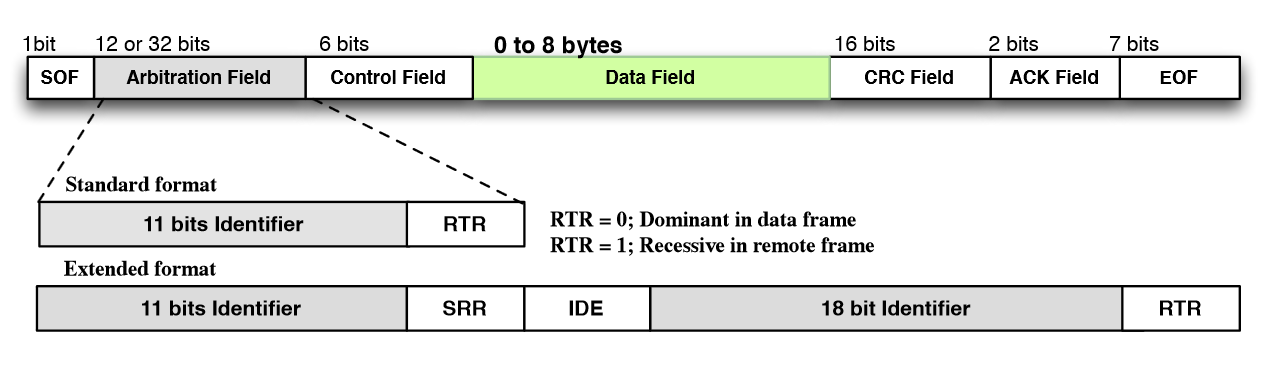
\includegraphics[width=4in]{frame}
  \caption {Structure of a data message frame in the CAN protocol [?]}
\end{figure}
    
    Every electric vehicle sold in the United States requires an outward-facing port on which listeners should be able to receive CAN messages conveying important diagnostic information about car malfunctions. Furthermore, most cars use a CAN bus internally to coordinate the activities of battery discharging, motor speed, dashboard updating, anti-lock braking management, and more. Interestingly, outside the automative sector, because of CAN's fault-tolerance, low cost, and lenient hardware requirements, CAN is used to link embedded systems in avionics, medicine, and military-grade weapon systems.\\
    
    Both essential and non-essential vehicle components communicate over a public CAN bus; this simplifies the complexity involved with having dedicated cross-component signal lines. An example network architecture is shown in Fig. 2.

\begin{figure}[h]
  \centering
  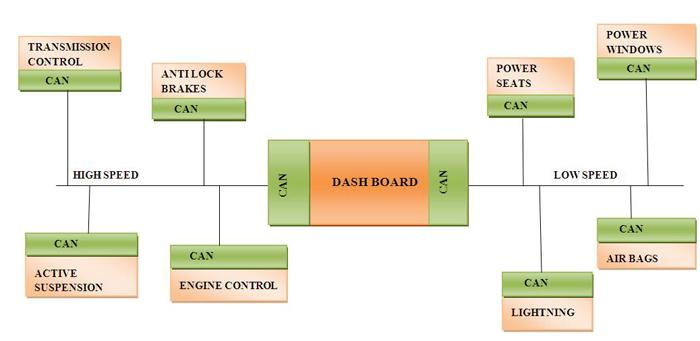
\includegraphics[width=4in]{car-network}
  \caption {Example intra-vehicular network architecture. Two separate CAN bus's handle different classes of behaviors. Messages sent on each bus are broadcast to every listening peripheral on that bus. The dash board listens in on both networks. [?]}
\end{figure}
    
    
    
    
  \subsection{Security Issues}
  As previously described, there are a number of known CAN exploits. These stem from the following characteristics of the CAN protocol:
  \begin{itemize}
    \item A CAN frame has no authentication field, enabling malicious nodes to send spurious commands to the motor controller and the like.
    \item The data field in a CAN frame is only 8 bytes long, making it difficult to add large-key security measures.
    \item ECUs do not always have the computational power necessary to perform cryptographic functions
    \item There is no authentication performed on the sender and receiver of a particular frame.
  \end{itemize}
  These flaws do not necessarily mean that CAN is poorly designed; again, it was intended to be a simple protocol that would work in isolation. They do mean, however, that it will be difficult to add authentication while still keeping within the parameters of the protocol.

\section{Threat Model}

A CAN network is susceptible to attacks that prevent transmission of authentic messages or forge disingenuous messages. In our design we aim to mitigate two major types of attack: \textbf{replay attacks} and \textbf{brute force attacks}. To more precisely define the capabilities and attack modes of our adversary, we define the following two CAN-based adversarial games:\\

\begin{framed}
\noindent \textbf{Bus-Frame Unforgeability Experiment} \\
On a bus-based network with $N$ nodes $n_1, n_2, ... n_N$, we define our scheme to be \textit{bus unforgeable} if for all PPT adversaries $A$, that $A$ succeeds after the following steps is negligible:\\

1. We choose $i$ key-pairs according to our key generation algorithm: $(SK_i, VK_i) \leftarrow KeyGen$. Limit $i \leq n$. Every node is assigned one $SK_i$. We provide every $VK_i$ and $N$ to $A$. All $N$ nodes on the network also get every $VK_i$. \\

2. $A$ is given access to an authentication oracle $Sign(SK, m, j)$ and a verification oracle $Ver(\sigma, m, j)$ for any message $m$ and any authentic signing agent $j \leq N$.\\

3. $A$ submits a challenge $(m',\sigma')$ to every $n_i$ with the restriction that $(m', \sigma')$ was queried with the verification oracle.\\

4. $A$ succeeds if for any $j$, $Ver(\sigma, m, j)$ returns True.
\end{framed}


The message-priority based arbitration of the CAN protocol allows for malicious nodes to continuously spam the network with high priority messages. Consequently, denial-of-service attacks are an unavoidable vulnerability of the CAN arbitration system. However, we will discuss an extension to our scheme that will allow users to more effectively respond to DOS attacks. Namely, this extension attempts to shutdown non-essential communication, offload communication to a back-up network, and identify the position of the malicious node within the compromised network \footnote{discussed in further detail in the paper's Analysis section}.

\section{Additional System Requirements}

For applicability reasons, we further constrained our design to fit an additional set of requirements:

\begin{itemize}
\item \textbf{Backwards compatibility}: Our system should ideally overlay across the current CAN structure. It is possible, for example, to extend the CAN message frame to have over 128 bits, allowing direct application of traditional authentication schemes, without dealing with the issues associated with small key sizes. However, fundamentally changing the structure of the CAN frame would prohibit our scheme from being applied to existing systems. Rather, we intend our system to fit within the existing standard CAN frame (not the extended CAN 2.0B frame), so that existing systems can easily apply our band-aid solution and achieve higher levels of security.
\item \textbf{Small number of shared keys}: There is no theoretical limit on the number of nodes connected to a CAN bus. In practice, we see anywhere from 1 to 127 nodes \cite{canopen}. Storing a flexible list of over one hundred 32-byte public keys is not insignificant for lightweight controllers, and we shall try to minimize this constant memory cost by grouping node keys (when appropriate and without compromising security).
    \item \textbf{Accommodate passive and active 3rd party devices}: It is unrealistic to assume a static network in a vehicle's CAN bus; peripherals may be added or removed from the network as time goes on. Diagnostic monitors, for example, might plug into a car's OBD2 port and passively read and authenticate messages from the motor controller. On the other hand, an added temperature sensor from a trusted manufacturer should be able to write authenticated messages to the bus without having reflash every CAN node.
\item \textbf{Low initialization, latency, and throughput overhead}: by adding our authentication scheme, the existing network should not see significant jumps in message latency or decreases in data throughput. The total amount of traffic in the network should increase by at most some constant factor.
\end{itemize}

\section{Previous Work}
A handful of symmetric key authentication and encryption schemes have been proposed in the past few years for in-vehicular networks. Few of them address all the requirements put forth in the aforementioned section. Two very powerful schemes developed by Verbauwhede et al., CanAuth and its successor LiBrA-CAN, rely solely on shared-key authentication, and accordingly, adding 3rd party passive listeners is not a supported operation\footnote{CANAuth and LiBrA-CAN were discovered in our literature search after substantial work had been done on developing the current scheme. Most the focus and goals of Verbauwhede et al.'s work and our work diverge significantly}. CanAuth does not support single source node authentication, but rather authenticates that the message is from some trusted source. LiBrA-CAN, as a progressive authentication scheme, requires $ n \choose s$ keys, $s$ some constant bounded by $n$. Practically, the number of keys required for this scheme could be quite large.\\

TESLA, another broadcast network alternative, is also a strong symmetric approach that uses delayed key disclosure. The protocol has been highly criticized for its need to store unauthenticated messages until their verifying key is disclosed [?]; the potential backup of messages makes TESLA susceptible to DOS attacks [?]. Later versions of TESLA have tried to address this but the attempted solutions have come with a significant increase in message latency [?].\\

Our literature search found two systems that apply AES-based encryption to a broadcast network, but neither are specific to vehicular CAN, nor do they achieve any sort of source authentication.

\section{Proposed Authentication Scheme}
    \subsection{Assumptions}
    Our algorithm, as will be described, assumes characteristics of the underlying CAN bus:
    \begin{itemize}
    \item There are three general variants of the CAN protocol: 
      \begin{enumerate} 
        \item the original fault-tolerant, low-speed protocol (CAN 2.0A)
        \item the high-speed protocol (CAN 2.0B)
        \item the flexible data-rate protocol (CAN FD). 
      \end{enumerate} 
        We will choose to overlay our authentication scheme on CAN 2.0A and safely assume lossless transmission over our CAN bus.
    \item One master exists with knowledge of the initial network topology and with a larger memory and computational capacity. This is a safe assumption since the most common electric vehicle designs includes at least one large ECU to manage motor movement and battery discharge dynamics.
    \end{itemize}
    We will discuss these assumptions (and how to generalize them) in our \textit{Analysis} section.
    \subsection{Big Picture}
    
    Our system is comprised of a public key and shared key authentication scheme. Despite its added computational cost, this choice to first apply a public-key scheme provides flexibility in our network architecture that pure shared-key does not. Specifically, third party peripherals added to the network are able to read and send authenticated messages by receiving and sending public key(s) over the bus. For example, added dashboard devices or OBD2 listener devices might be added over the course of a vehicle's lifetime. We do all authentication of messages through the shared key channel, set up by the public key infrastructure. We choose a shared-key authentication system to do the heavy lifting in real time to minimize the overhead of public key authentication during time-critical messaging.\\
    
    There are two high-level steps for producing and verifying signatures in our scheme:\\
    
    \begin{enumerate}
    \item \textit{Initialization\footnote{Likely to take place during the initial assembly of the system at the OEM plant}:} Every node is assigned exactly one (not necessarily unique\footnote{See our section on Shortening the Public-Key Directory}) secret-key, public-key pair with which it will sign messages that it broadcasts. A sufficiently powerful ECU designated as a trusted master must receive a unique key pair. Furthermore, every node is given a unique ID. Every node is responsible for storing and maintaining a directory of public-keys to the extent that its memory has capacity (more on this in future sections).\\
    
    \item \textit{During Runtime:} Any node that decides to broadcast in an authenticated fashion will set up an authenticated \textbf{send channel}. Recipient nodes that are interested in listening to that sender node listen in on this channel. As we will describe later, the basis for each channel is an HMAC chain. (see section \ref{sec:hmac}). All messages sent across this send channel are source authenticated and there are  $O(n)$ channels running simultaneously. 
    \end{enumerate}
    
\begin{figure}[h]
  \centering
  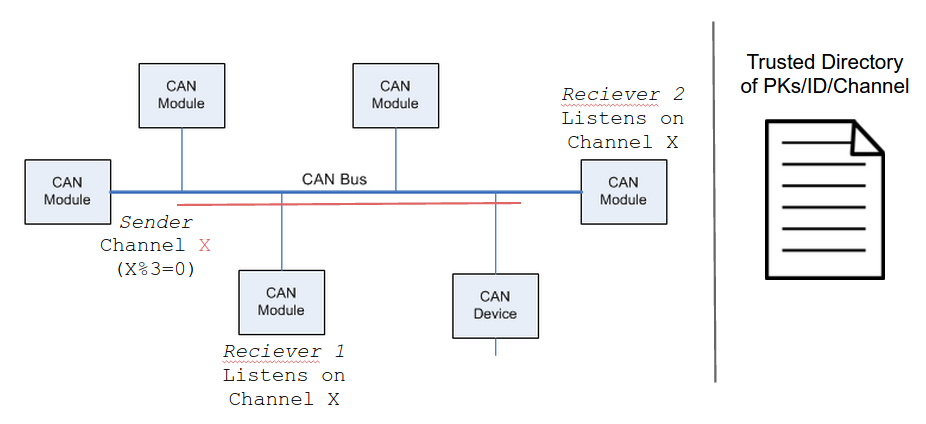
\includegraphics[width=0.5\textwidth]{channelX}
  \caption {Example of a secure channel from the sender (leftmost node with unique ID $X$) to the bus. The broadcast message IDs associated with this channel is some integer $n$ where $n\equiv X$ (mod total number of nodes)}
\end{figure}
    
    \subsection{Basis of Channels}
    \label{sec:hmac}
    
    \subsubsection{Authentication by HMAC Channels}
    Each channel is a method to produce authentication tags for the set of $n$ messages that a sender wishes to broadcast. To produce these authentication tags, we use an HMAC chain: \\
    
\begin{figure}[h]
  \centering
  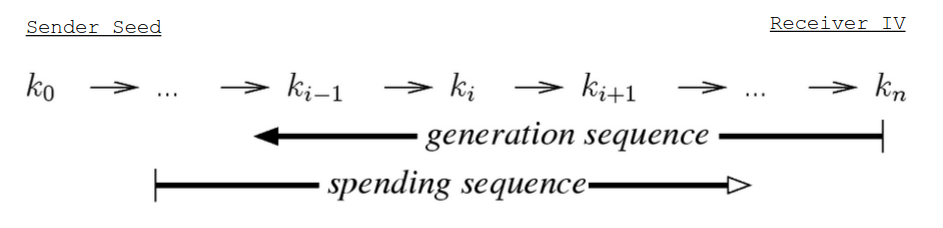
\includegraphics[width=4in]{hchain}
  \caption {HMAC chain used for verification of a message}
\end{figure} 
    
    Specifically, the sender chooses a random (secret) seed and 256-bit channel key $K$ and computes $tag_i = HMAC(K,tag_{i-1})$ for all $0<i \leq n$. The sender sends a message onto the bus with $tag_n$, $K$, and his RSA signature for the previous two values. The receiver verifies that the initial chain value $tag_n$ and $K$ have not been tampered with. The authentication tag $t_i$ for every message $m_i$ is $m_i \xor tag_i$. Every receiver verifies that a message $t_i,m_i$ is from the claimed source by retrieving its saved $K$ and $t_{i+1},m_{i+1}$ (the previous tag, message pair) by verifying: $$HMAC(K,t_i \xor m_i) = t_{i+1} \xor m_{i+1}$$
    
    We choose to use an HMAC authentication scheme rather than merely using a one-way hash in the hash chain to prevent replay attacks. It may be common for a node to transmit the same message multiple times. Because our tag size must be less than 4 bytes, tags must necessarily repeat after a small number of messages. With high probability,  the same message-tag pair will be sent across the network in two different channels. Using a static hash function means that an adversary could memoize each transmitted chain and replay the chain once he finds a repeat message-tag pair. Keyed hash functions offered by HMAC allow every chain to be unique. \\
    
    After consuming the entire chain, a new chain must be created in the same manner. The security properties of hash chains have been explored thoroughly in other works \cite{hmacsecurity}.
    
    \subsubsection{Scheme Frame Structure}
    Unfortunately, direct application of the authentication scheme described in this paper is not possible with the CAN protocol. The protocol is intended to be implemented as a layer on top of the CAN protocol, meaning that we need to fit the data into CAN data frames. Here we describe a way of allocating the frame payload structure to accommodate the scheme. We put the authentication tag in the same frame as the message (instead of designating separate authentication frames and message frames) to avoid the possibility of building up queues of message frames waiting for their authentication frames.\\
    
    For the channel setup messages, we designate a specific message ID requirement: the first bit in the message ID must be 0. Each channel setup message must transmit part of the channel HMAC key, the initial value $tag_n$, the channel source node ID, and a signature for the aforementioned values:\\
   
\begin{figure}[h]
  \centering
  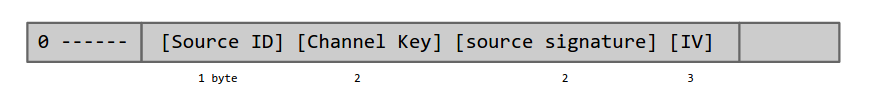
\includegraphics[width=4in]{channel-setup-frame}
  \caption {Diagram outlining the general message frame structure for messages devoted to setting up a channel. Given our 256-bit HMAC key size, we expect 128 messages to be devoted to setting up each channel upon vehicle startup.}
\end{figure}

    After interested receivers receive the complete set of channel setup messages, the node is able to verify the authenticity of the aggregate data by validating the signature \footnote{The authors recognize that a denial of service attack may be possible in this stage by indiscriminate sending of incorrect-signature channel setup messages (which the receiver goes through and verifies). We discuss more in the paper's Analysis section}. If authentic, it saves channel key and first tag for use in validating data transmission messages.\\

     For the data transmission messages on an already setup channel, we designate a different message ID requirement: the first bit in the message ID must be 1. Each data message must transmit part of the source ID, the data segment, and its corresponding tag: \\

\begin{figure}[h]
  \centering
  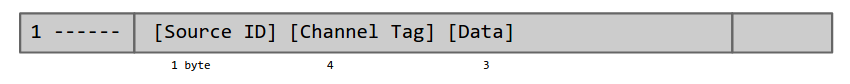
\includegraphics[width=4in]{data-frame}
  \caption {Diagram outlining the general message frame structure for messages devoted to transmitting data on a channel.}
\end{figure} 
    
    \subsubsection{Other Scheme Details and Addendums}
    \textbf{Linking Message IDs with Channel Identities}\\
    
    Nodes on a CAN bus are generally interested in listening to a subset of other nodes (e.g. the motor is interested in listening to the motor controller, not the dashboard). As such, it makes sense to use the existing CAN message ID filtering to achieve this sort of selective listening of the bus. To integrate our notion of channel listening with this idea, we need to think carefully about how to assign each message ID. We are constrained by the fact that lower message IDs get priority on a CAN bus, and to ensure fair sending characteristics between nodes, we need to integrate some degree of randomness to each message ID assignment.\\
    
    Our proposed solution first assigns each node $n$ in the original network a unique ID. For simplicity, if there are $N$ nodes total in the initial network, assume that every node is assigned a distinct integer $i$ in $0\leq i < N$. There are 10 bits to encode the message ID \footnote{There are eleven bits in practice, but we occupied the first bit to distinguish channel setup messages}, so our message ID is in the range $[0,2^{10})$. For every channel, there is exactly one sender on that channel, and one node ID. The last ten bits of the message ID for node $i$'s sending channel is any random $R$ where $R \equiv i$ mod $N$. This setup ensures that channels don't interfere and that there is roughly similar probability that any channel has precedence over another channel.\\
    
    \textbf{Changes to the Bus \& Public-Key Directory} \\
    
    New nodes added after initial network setup are able to authenticate messages found on the bus after a channel refresh. We assume that such '3rd party' nodes have access to the directory of network public keys, perhaps available by the OEM \footnote{original equipment manufacture} of the original network. Alternatively, messages may be sent to a designated master to query for specific entries in the public key directory. In the next section, we will briefly discuss how this may be useful.\\
    
    A refresh of the public-key directory (for whatever reason, perhaps the network has sufficiently changed, or certain private-public key pairs have been compromised), may be arbitrated by the master. Changes to the directory should not be allowed without prior authentication (a malicious node may spoof an authentic one), but it is possible to encode a scheme whereby the master arbitrates authenticates change requests to the directory and broadcasts those messages in an authenticated fashion. We do not implement this protocol addendum in our testing framework, but we do note that our scheme allows for such an extension.\\
    
    \textbf{Compressing the Public-Key Directory} \\
    
    Memory limitations are discussed in more detail in \textit{Analysis}, but it is worth noting that should the $O(n)$ storage of public keys per keys become a bottleneck, it is possible to compress the PK directory. Specifically, notice that two or more trusted nodes may share a channel (if their set of recipients is the same, and exact source verification between the two is not needed). Furthermore, only sending nodes need to possess public-private key pairs. In a generic car model, passive listeners comprise a large quantity of the nodes on the network: the dashboard, motor, light systems, and more.\\
    
    In super lightweight nodes, it may be that only storage of $O(1)$ keys is possible. In this case, it is possible to offload authentication work to a trusted master, redirect traffic to the master, and receive and authenticate messages only from the master. In our testing framework, we assume that each node's memory capacity exceeds the requirements for PK directory storage, so we leave this addendum unimplemented.\\
    
    The authors note that it takes a few steps to modify the proposed scheme to conceal P2P-channel traffic. Using the public key of the recipient, it is possible to send and transmit an AES-256 CBC encryption similar to how we establish and transmit channel keys. From there, we encrypt and send data over the channel.
    
    \section{Analysis}
    To determine if our protocol met our design goals we performed analysis both theoretically and practically using a homebrew CAN software simulation. In our analysis, we endeavoured to characterize the security that our protocol affords the users and the additional costs that must be incurred to achieve said security.

    \subsection{Theoretical Analysis}
    \subsubsection{Brute Force Attacks} 
    Using the scheme described in this paper, an adversary has a space of 32 bits to brute force potential tags for a certain message. Due to the nature of HMAC authentication, the tag necessary to validate any particular message will not be constant, so attempting to validate all possible tags for a certain message is not guaranteed to get a fraudulent message accepted. However, if an adversary guesses a random tag for some message, there is a $2^{-32}$ chance of that message being accepted. Thus the expected number of message transmissions from an adversary until a fraudulent message is accepted is $2^{32}$. CAN buses can run at a variety of bit rates, most typically 250kbs. With the message size being 108 bits this gives $\frac{250,000}{108}$ messages per second. We assume our adversary is able to transmit on the order of one message per one hundred message cycles; faster than this would congest the bus and would be considered a DOS attack, addressed above. With these assumptions we have that the expected time to successful brute force is $\frac{2^{32}*108*100}{250000}$ seconds or approximately six years.
    
    \subsubsection{Memory}
    Due to the nature of our public key system, each node must maintain the values of its private key and the public keys of all trusted nodes in the network. Additionally, for each active channel, each node must maintain the hash value at the current head of the chain for validation along with the hash key. In the worst case this gives us $O(n)$ memory overhead per node, $O(n^2)$ across the entire network. Many common modern car architectures use  approximately 70 CAN nodes. With 256-bit public and private key pairs, 32-bit authentication tags, and 256-bit HMAC keys, the memory overhead incurred by each node in a network with $n$ nodes is $(256+32+256)n = 544\text{ bits }= 68\text{ bytes}$ in the worst case. Thus, in a typical network of 70 nodes, our protocol requires each node to store an additional 4760 bytes of information. A common specification for micro-controllers deployed on CAN networks provides 12MB of random access memory \cite{analog2002}; supporting the memory requirements for our protocol.
    
    \subsubsection{DOS Attacks} Denial-of-Service attacks are a inherent weakness of CAN-based networks. The message arbitration scheme on the CAN bus permits nodes to pull the differential pair of CAN bus wires continuously high (writing an infinite logical 0). A malicious node may drive the bus to a static state by continuously transmitting high priority messages in this way, shutting down communication between non-malicious nodes. No network algorithm can circumvent this, and the bus is compromised. We imagine that dealing with such an attack would require some sort of overlay logic. The aforementioned attack is simple to detect by any node, so it is possible to have an overlay network that connects every pair of nodes in a small, predetermined set of trusted nodes. In case of a bus hijacking, the network falls back to the overlay network and maintains only vehicle critical processes. Alternatively, it may be possible to design hardware additions along the bus that are able to (1) monitor transmissions and small voltage gradients along the bus and (2) cut off subsets of nodes along the bus. This allows for fast detection when a node is attempting to push a malicious amount of traffic to the bus, and rapid disconnection of the malicious node. The implementation of such an arbitration scheme is beyond the scope of this paper. \\
    
    We imagine that an alternative denial-of-service attack may occur during transmission of channel setup messages. A malicious node may inject a false signatures message and invalidate the entire set of channel setup messages. Again, detection of such an attack is straightforward; nodes experiencing such a DOS experience many failed channel setup attempts. Elimination of this issue might require a less secure small authentication tag for the data segment in every single channel setup frame (as opposed to our sender's RSA signature spread across multiple frames).
    
    
    \subsection{Simulation}
    In order to analyze how our protocol would affect traffic on an active CAN implementation, we chose to develop a CAN simulator in software \footnote{Our software can be downloaded from our GitHub repository at \url{https://github.com/MatthewChang/CANSim}} which could support an implementation of our protocol.
    
    \subsubsection{Implementation and Preliminary Results}
    The system was designed with the contents of the message fields in each CAN frame as the smallest atomic unit. We chose to abstract out bus voltages and similar hardware reliant components as such details would be subject to change given any specific CAN implementation. Each virtual CAN node operates on a synchronized clock which ensures that for every clock cycle, each node on the network has both read and write access to the shared bus once and only once. This guarantee allows us to model a lossless CAN protocol by specifying that during its access time on the bus, each node obey standard CAN arbitration rules based on message identification.\\
    
    With a working simulation of the underlying CAN network, we were able to implement our proposed secure protocol as an abstracted message passing system. For generating public and private keys we used a third party library Python-RSA \cite{http://stuvel.eu/rsa}. We used the in-built Python \texttt{\href{https://docs.python.org/3/library/hmac.html}{hmac}} and \texttt{\href{https://docs.python.org/3/library/hashlib.html\#module-hashlib}{hashlib}} libraries for our implementation of SHA-256 and other necessary cryptographic primitives.
    
    \subsubsection{Traffic Overhead}
    To model traffic we created a virtual CAN network with nodes to simulate standard car components (e.g. steering wheel, motor controller, brakes, dashboard, etc...) During each clock cycle, nodes had a random chance to queue up messages to be broadcast on the bus. Running our simulation using both the (unauthenticated) standard CAN-A protocol, and the authenticated CAN protocol described in this paper, we found the following on a series of tests run for 100 simulated clock cycles. We logged the throughput as the total number of messages successfully transmitted across the bus and logged the latency as the number of clock cycles between the time a message was queued, and the time it was acknowledged/verified by all nodes in the network. 
    
    \begin{figure}
    \centering
    \begin{tabular}{|c|c|c|}
    \hline
    & Throughput & Average Message Latency \\ \hline
    CAN-A & 78 & 10.2\\ \hline
    Authenticated CAN & 88 & 32.7 \\ \hline
    \end{tabular}
    \caption{Throughput and latency results from software simulation}
    \end{figure}
    
    \subsection{Concerns}
    Our proposed authentication scheme has a handful of issues that we see as areas of future work. First, we aim to reduce the time it takes for a message to reach the bus and be read by bus nodes (our 'message latency'). Directly related, is the high amount of additional traffic (that any authentication scheme) that is added to the network. Transmitting any sort of authentication information increases the total amount of traffic on the bus, and increases the time that messages must wait before they are able to occupy the bus.\\
    
    One important aspect of our scheme that we still need to fully wrinkle is transmission of acknowledgement of channel setup. The current implementation has senders assume that channel setup is successful after all setup messages have been sent, but as noted, this is susceptible to injection attacks. Ideally, we'd have an authenticated acknowledgement, or self-authenticating channel setup message. We can achieve the former by initially setting up of all possible two way channels, and relying this to acknowledge any new channels that replace old channels. The downside to this solution is that this largely invalidates our suggested optimizations, and would add a fair bit of computational overhead. Alternatively, we could sign every message frame with our public-private key pair, and truncate to fit into the frame. We'd need to ensure that brute force attacks are still infeasible.\\
    
    Finally, as mentioned before, our scheme, as implemented, does not address DOS attacks. We have suggested work-arounds, but these are neither complete nor tested.

\section{Conclusion}
  Our results were promising and showed that it would be possible to add an authentication scheme based on public keys and shared keys to the CAN protocol. Our implementation suffers from a few limitations and we had to make tradeoffs in order to meet all of the requirements we set out for ourselves. Future work would involve testing our implementation on actual hardware and measuring the effects of our changes on latency and overall traffic in real life situations.

\bibliographystyle{plainnat}
\bibliography{references}

\appendix

\end{document}

